\section{Referencia de la Clase Articulo\-List\-Sub\-Form}
\label{classArticuloListSubForm}\index{ArticuloListSubForm@{ArticuloListSubForm}}
Clase que maneja el detalle de la lista de art\'{\i}culos.  


{\tt \#include $<$articulolist.h$>$}

Diagrama de herencias de Articulo\-List\-Sub\-Form\begin{figure}[H]
\begin{center}
\leavevmode
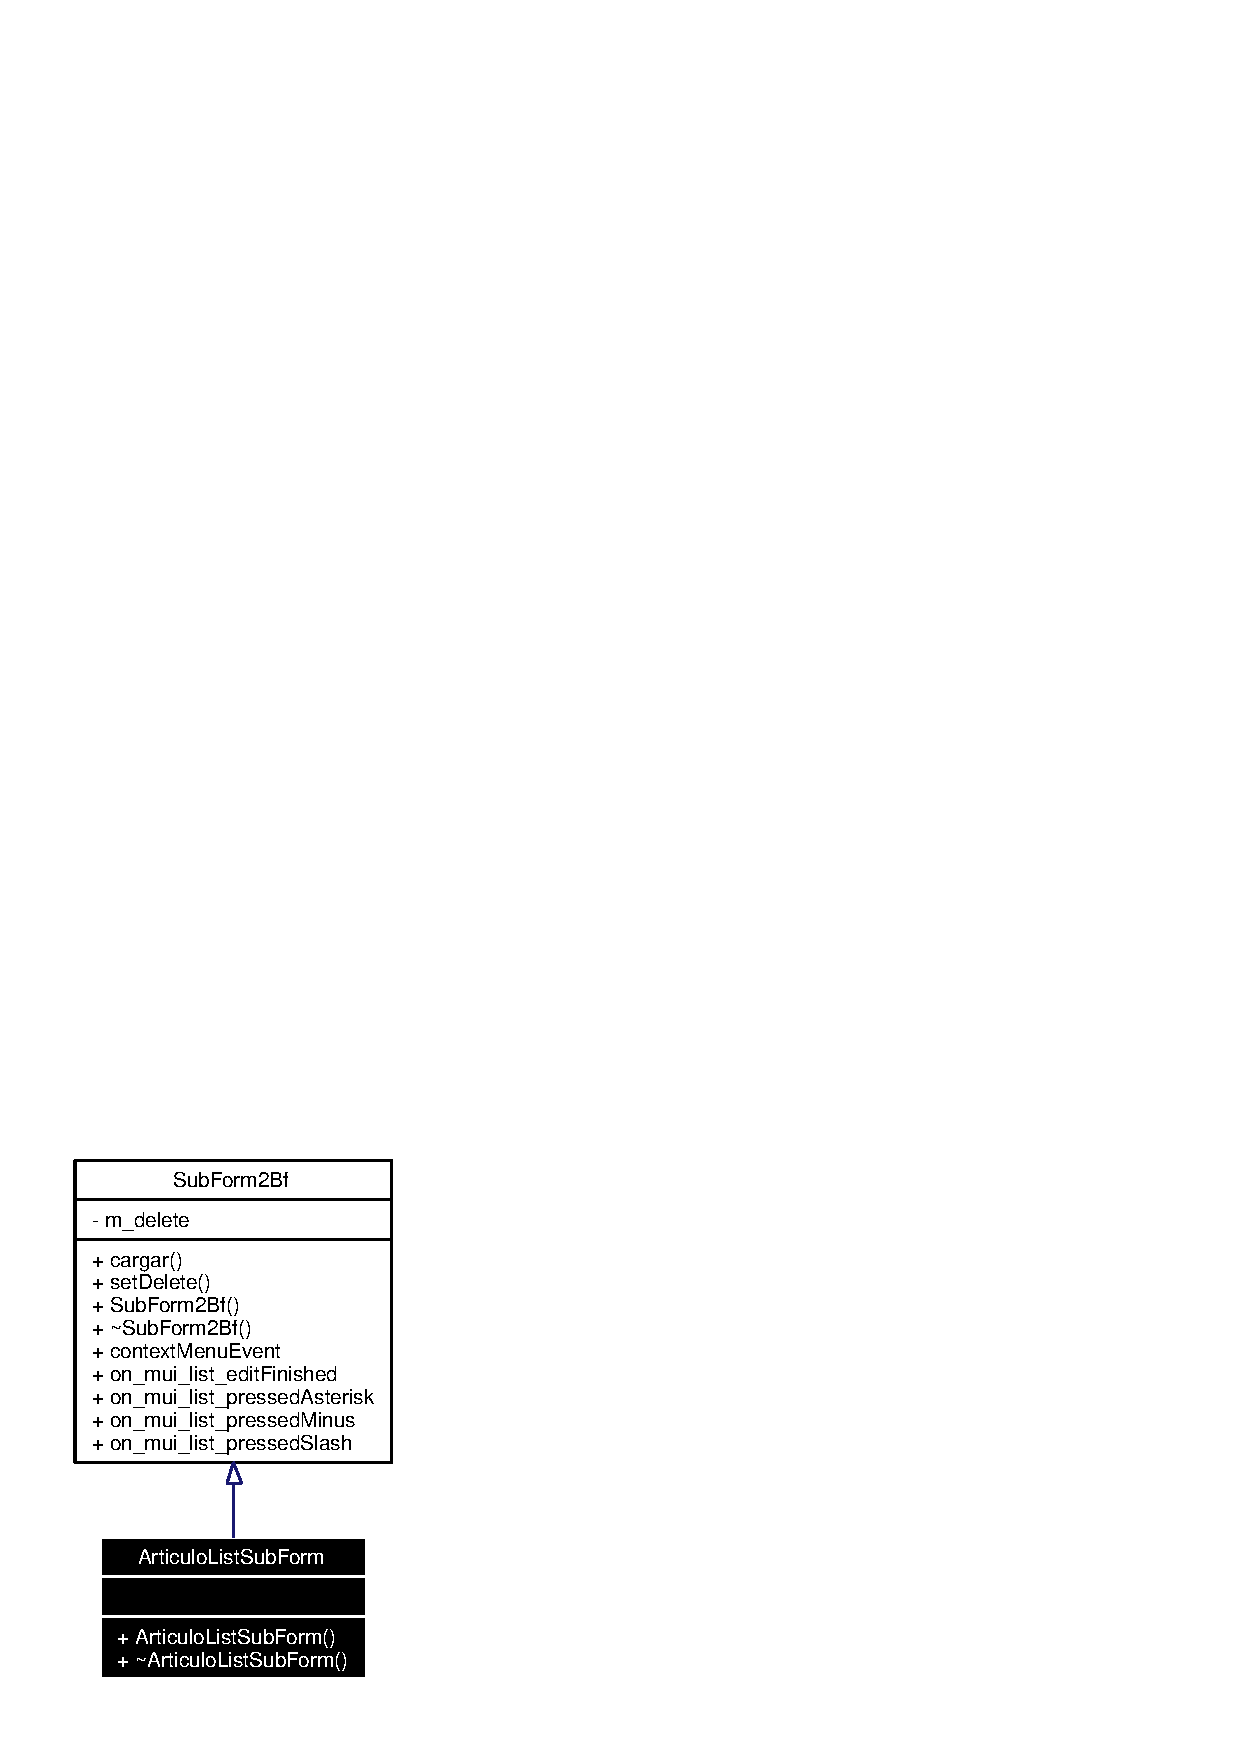
\includegraphics[width=94pt]{classArticuloListSubForm__inherit__graph}
\end{center}
\end{figure}
Diagrama de colaboraci\'{o}n para Articulo\-List\-Sub\-Form:\begin{figure}[H]
\begin{center}
\leavevmode
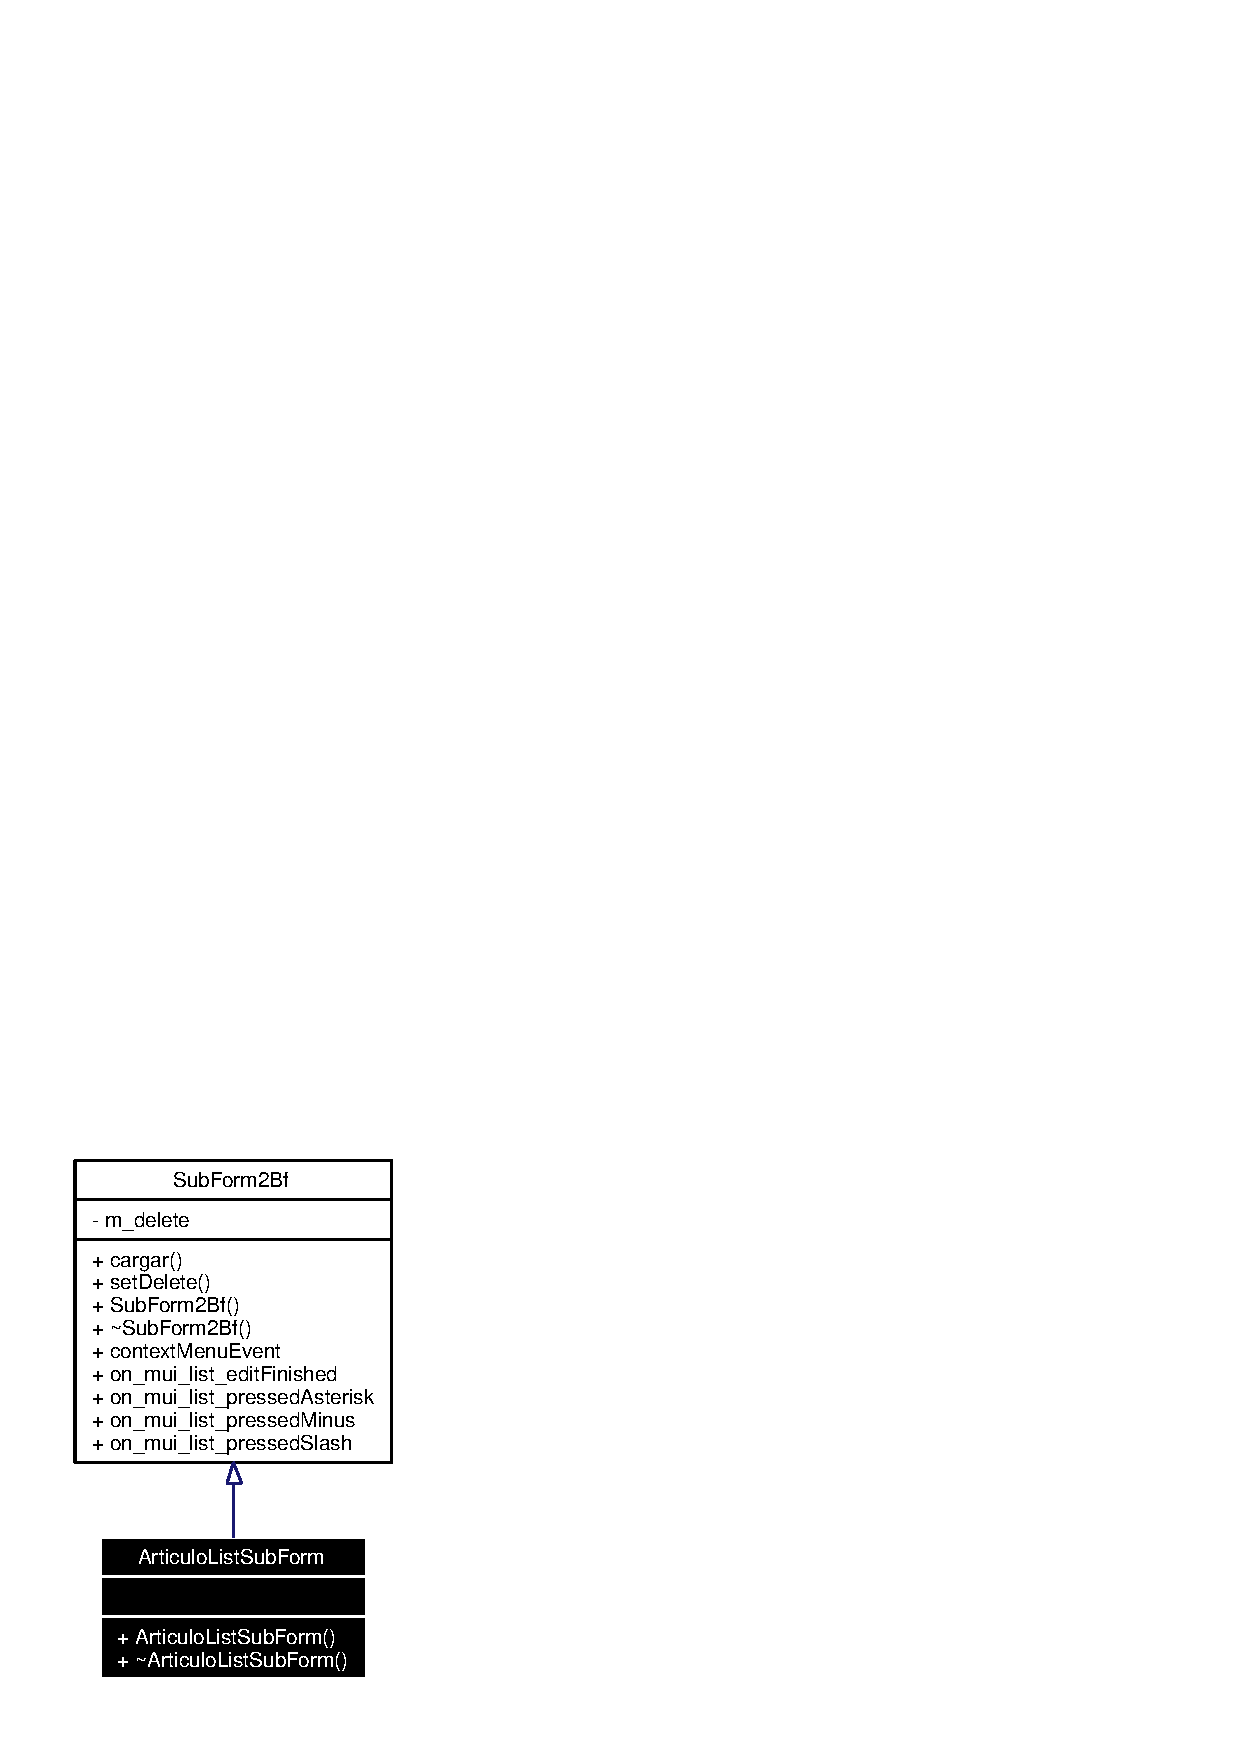
\includegraphics[width=94pt]{classArticuloListSubForm__coll__graph}
\end{center}
\end{figure}
\subsection*{M\'{e}todos p\'{u}blicos}
\begin{CompactItemize}
\item 
{\bf Articulo\-List\-Sub\-Form} (QWidget $\ast$parent=0, const char $\ast$name=0)
\end{CompactItemize}


\subsection{Descripci\'{o}n detallada}
Clase que maneja el detalle de la lista de art\'{\i}culos. 



\subsection{Documentaci\'{o}n del constructor y destructor}
\index{ArticuloListSubForm@{Articulo\-List\-Sub\-Form}!ArticuloListSubForm@{ArticuloListSubForm}}
\index{ArticuloListSubForm@{ArticuloListSubForm}!ArticuloListSubForm@{Articulo\-List\-Sub\-Form}}
\subsubsection{\setlength{\rightskip}{0pt plus 5cm}Articulo\-List\-Sub\-Form::Articulo\-List\-Sub\-Form (QWidget $\ast$ {\em parent} = {\tt 0}, const char $\ast$ {\em name} = {\tt 0})}\label{classArticuloListSubForm_a0}


============================================================================= SUBFORMULARIO ============================================================================= 

La documentaci\'{o}n para esta clase fu\'{e} generada a partir de los siguientes archivos:\begin{CompactItemize}
\item 
articulolist.h\item 
articulolist.cpp\end{CompactItemize}
